\documentclass{beamer}

\usepackage{multicol}
%\usepackage[dvipsnames]{xcolor}
\usepackage{graphicx}
\usepackage{pifont}
\usepackage{multirow}
\usepackage{ragged2e}
\usepackage{changepage}

\usepackage{wrapfig}

% Grafici
\usepackage{graphicx, booktabs, wrapfig, pdfpages}

\usepackage[framemethod=tikz]{mdframed}
\usepackage[outline]{contour}
\usepackage[ labelfont=bf, labelsep=period, margin=0.5in]{caption}\usepackage{pdfpages}
\usepackage[labelfont=bf, labelsep=period, margin=0.5in]{caption}

\usepackage{upgreek} %per scrivere mu non corsivo (\upmu)

% Use Unipd as theme, with options:
% - pageofpages: define the separation symbol of the footer page of pages (e.g.: of, di, /, default: of)
% - logo: position another logo near the Unipd logo in the title page (e.g. department logo), passing the second logo path as option 
% Use the environment lastframe to add the endframe text
\usetheme[pageofpages=of]{Unipd}

\title{Proprietà dei candidati Muoni del Trigger L1 di CMS}
%\subtitle{Demonstrating how to use the Unipd theme}
\author[La Rovere Francesco]{La Rovere Francesco}

\date{9 Dicembre, 2024}

\AtBeginSection[]
{
  \begin{frame}
  \Large

    \frametitle{Indice analitico}
    \tableofcontents[currentsection, subsectionstyle=show/shaded]
  \end{frame}
}

\begin{document}
\footnotesize

% Make the title page
\frame{\titlepage}

\section{Introduzione}

\begin{frame}{Il Large Hadron Collider}

Situato a Ginevra, Svizzera, il Large Hadron Collider è il più grande acceleratore di particelle mai costruito. 

\vspace{0.5cm}
\begin{columns}
    \begin{column}{0.65\textwidth}
        \begin{itemize}
            \setlength{\itemsep}{10pt} % Aumenta lo spazio tra gli item
            \item Collisione di particelle a $\sqrt{s} \approx 14$ TeV
            \item Luminosità istantanea $\mathcal{L} = 2 \times 10^{34}cm^{-2}s^{-1}$
            \item Rate di interazioni 40MHz $\rightarrow$ 25ns tra le collisioni
            \item Fasci di particelle formati da pacchetti discreti di protoni
        \end{itemize}
    \end{column}
    \begin{column}{0.35\textwidth}  
       %\scalebox{0.26}{\includegraphics{Immagini/LHCPath.png}}  
    \end{column}
\end{columns}

\end{frame}


\begin{frame}{Il Compact Muon Solenoid}

\begin{columns}
    \begin{column}{0.45\textwidth}
    \end{column}
    \begin{column}{0.55\textwidth}  
       %\scalebox{0.15}{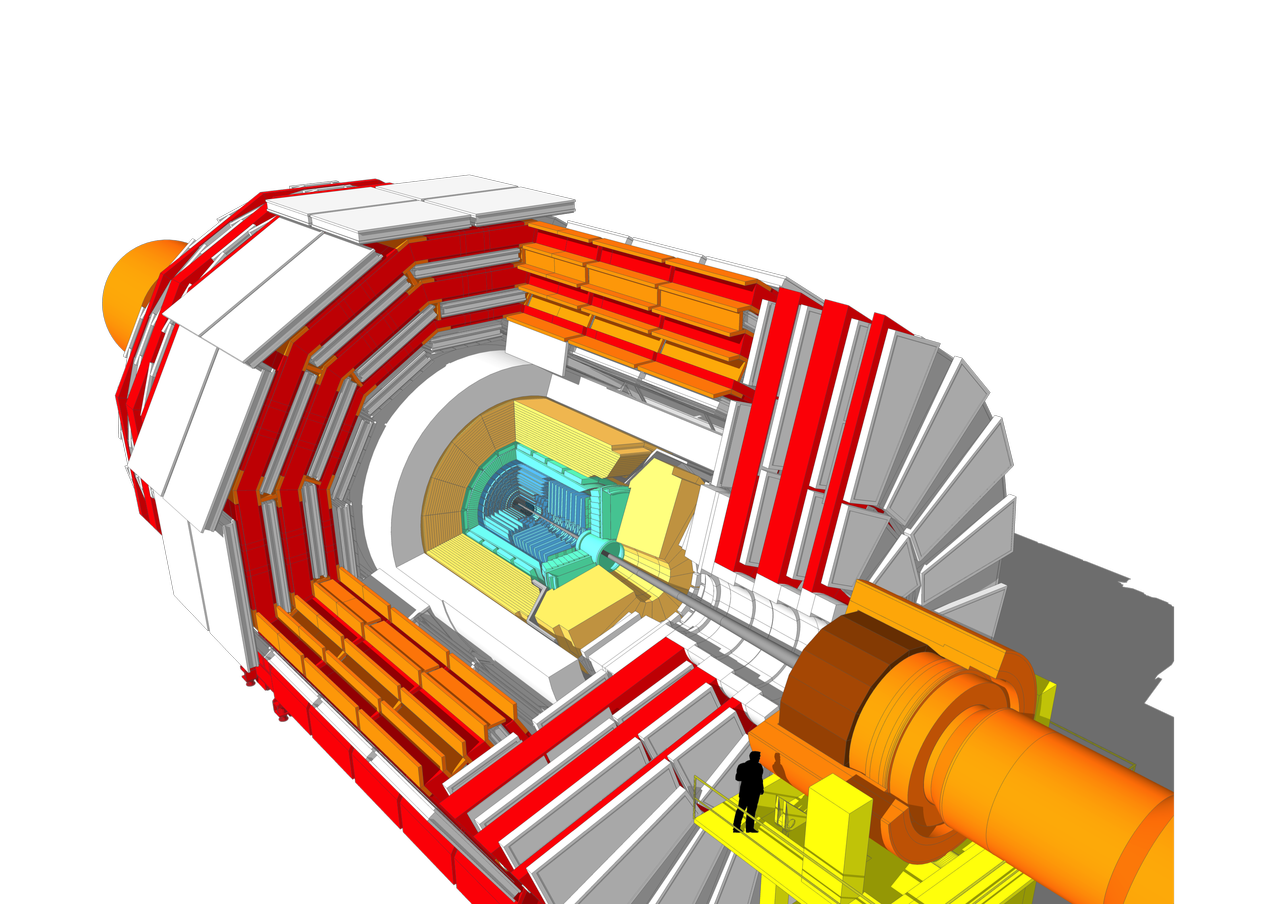
\includegraphics{Immagini/CMS.png}}  
    \end{column}
\end{columns}

\end{frame}

\begin{frame}{CMS: struttura}

\begin{columns}
    % Colonna di testo (sinistra)
    \begin{column}{0.5\textwidth}
        Panoramica della struttura di CMS:
        \begin{itemize}
            \item Silicon Strip Trackers
            \item Calorimetro Elettromagnetico
            \item Calorimetro Adronico 
            \item Solenoide Superconduttore 
            \item \textbf{Camere Muoniche}
                \begin{itemize}
                    \item Regione di barrel
                    \item Regione di overlap
                    \item Regione di endcap
                \end{itemize}
        \end{itemize}

        Le camere muoniche sono formate da:
        \begin{itemize}
            \item 4 Station
            \item 12 Sector
            \item 5 Wheel
        \end{itemize}
    \end{column}

    % Colonna di immagini (destra)
    \begin{column}{0.5\textwidth}
        \centering
        %\scalebox{0.10}{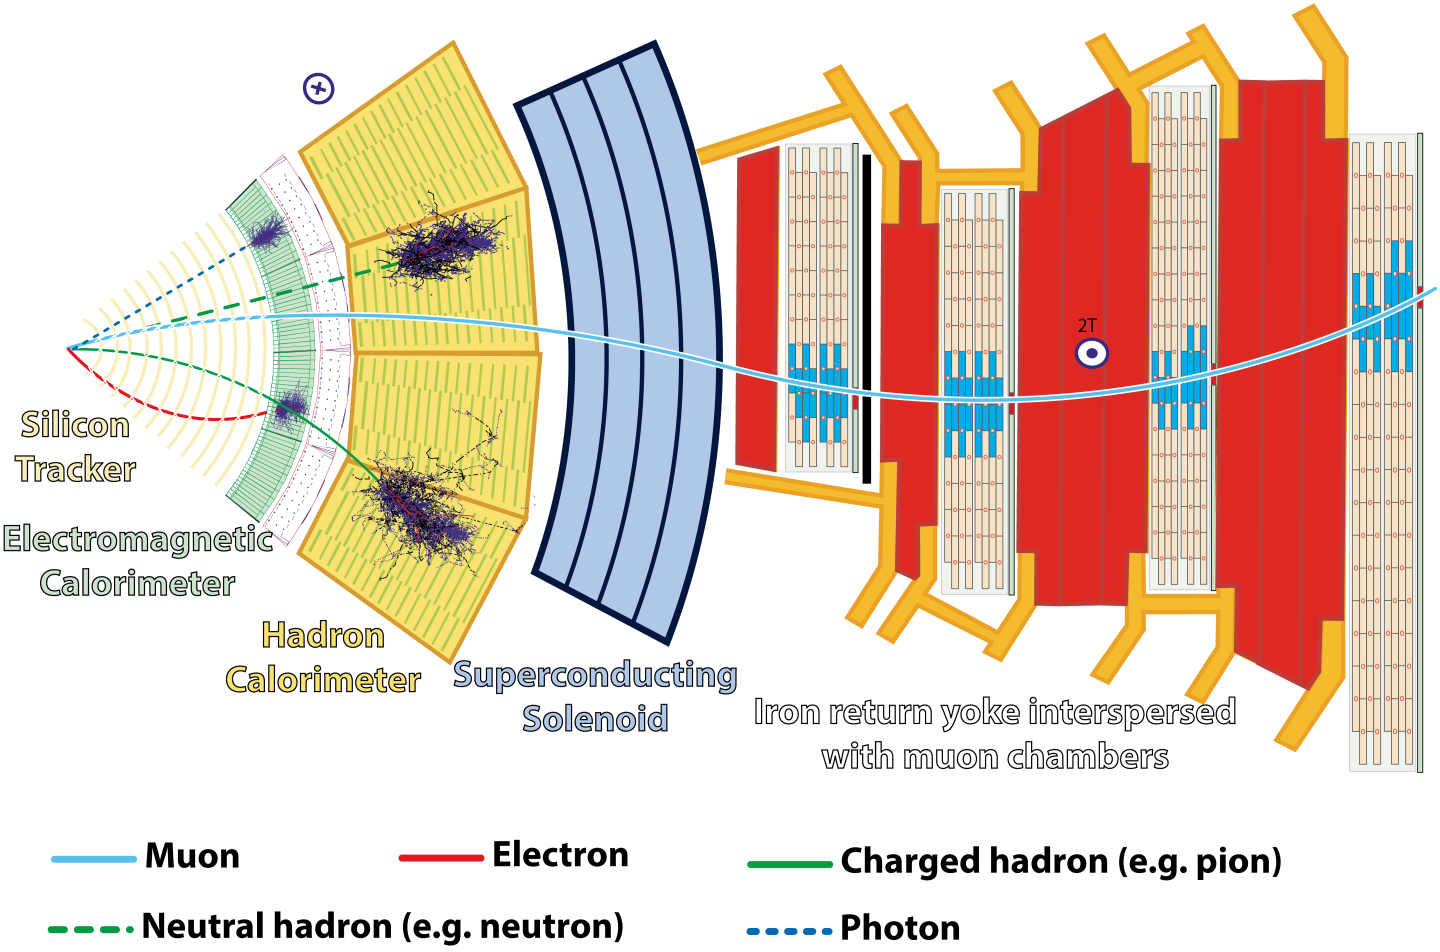
\includegraphics{Immagini/CMS slice.png}} 
        %\scalebox{0.20}{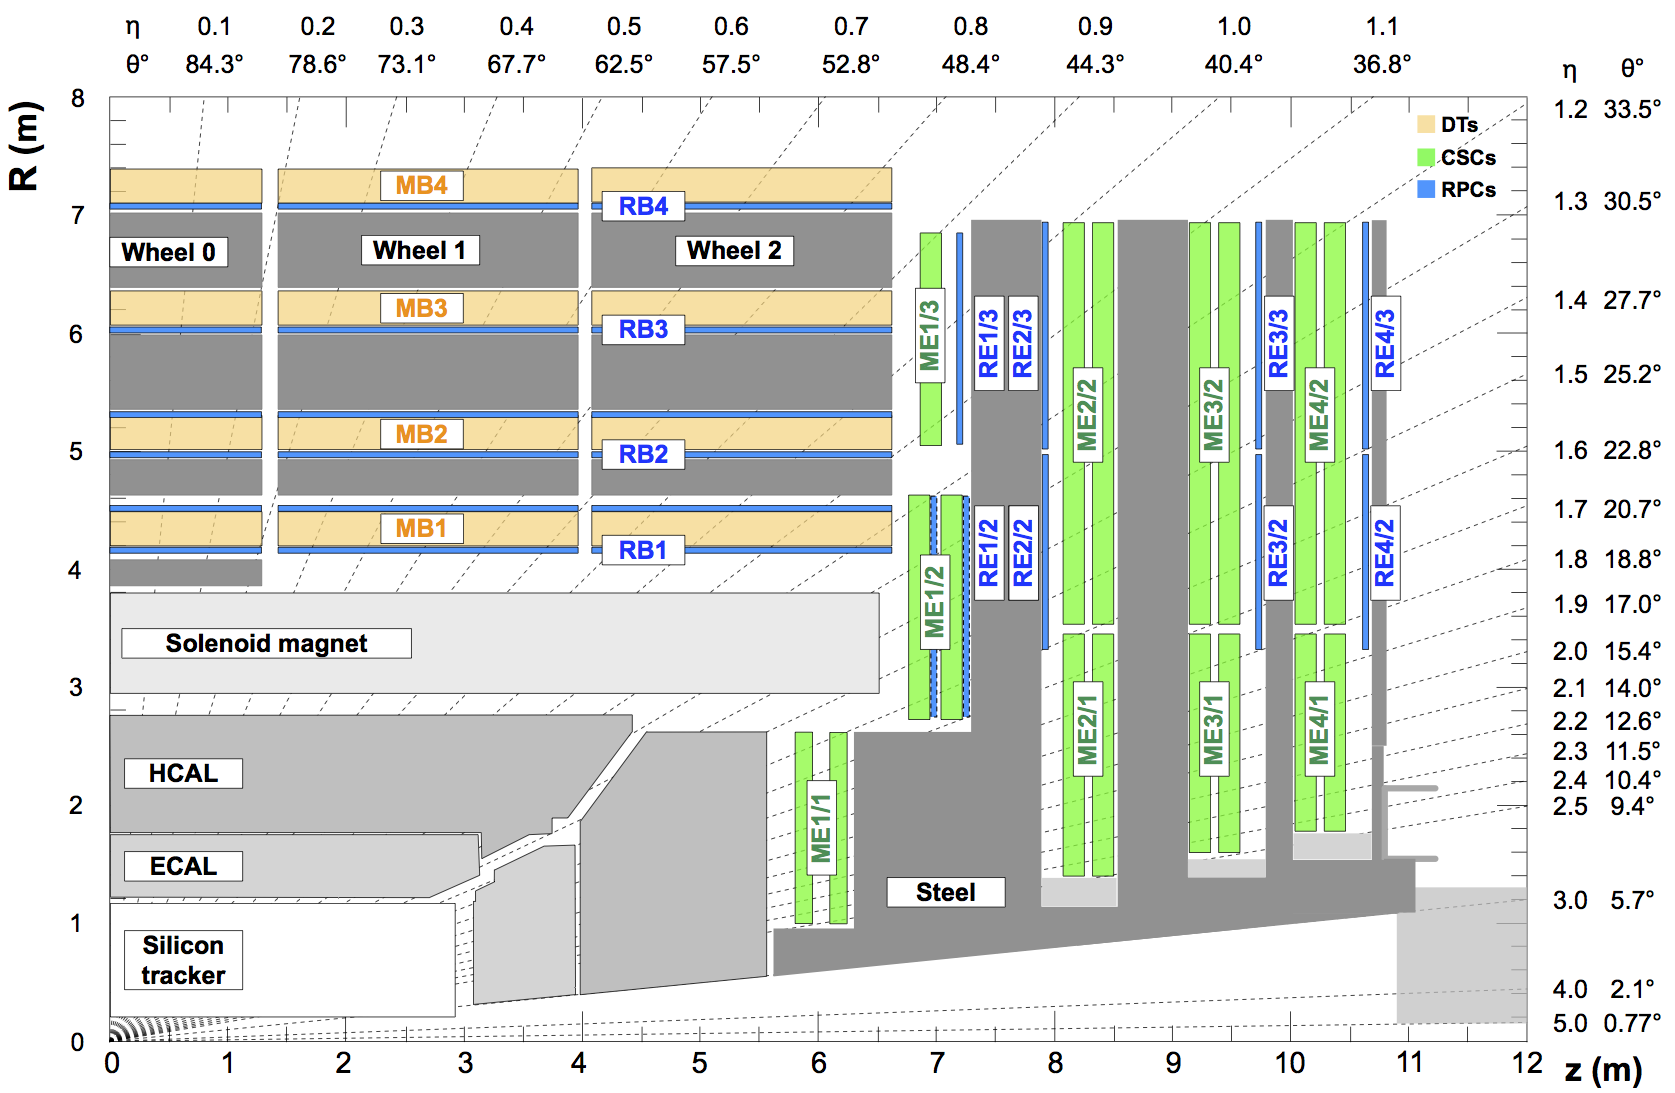
\includegraphics{Immagini/CMSEtaView.png}} 
    \end{column}
\end{columns}

\end{frame}


\begin{frame}{CMS: camere muoniche}

\begin{columns}
    % Colonna di testo (sinistra)
    \begin{column}{0.6\textwidth}
    \begin{itemize}
        \item Regione di barrel, $|\eta| < 1.2$:
        \begin{itemize}
            \item Eventi di background minimi
            \item Sono impiegati DT e RPC
        \end{itemize}

        \item Regione di endcap, $1.2 < \eta < 2.4$:
        \begin{itemize}
            \item Eventi di background elevati
            \item Sono impiegati RPC e CSC
        \end{itemize}
    \end{itemize}


    \end{column}

    % Colonna di immagini (destra)
    \begin{column}{0.4\textwidth}
        \centering
        %\scalebox{0.22}{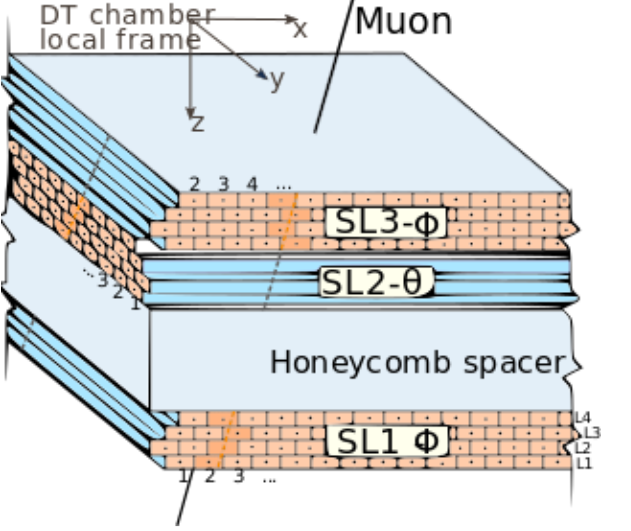
\includegraphics{Immagini/DriftTubes.png}} 
        \vspace{0.2cm}
        %\scalebox{0.4}{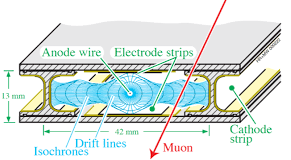
\includegraphics{Immagini/DriftTubes2.png}} 
    \end{column}
\end{columns}

    
\end{frame}



\begin{frame}{CMS: sistema di Trigger}

\begin{columns}
    % Colonna di testo (sinistra)
    \begin{column}{0.5\textwidth}
        Impossibile gestire il flusso di informazioni $\rightarrow$ sistema di Trigger:
        \begin{itemize}
            \item Level 1 Trigger
            \begin{itemize}
                \item Riduzione tasso di eventi da 40MHZ a 100kHz
            \end{itemize}
            \item High Level Trigger
            \begin{itemize}
                \item Riduzione tasso di eventi da 100kHz a $\approx$ 1kHz
            \end{itemize}
        \end{itemize}

    \end{column}

    % Colonna di immagini (destra)
    \begin{column}{0.5\textwidth}
        \centering
        %\scalebox{0.2}{\includegraphics{Immagini/TriggerNic.png}} 
        \vspace{0.2cm}
        %\scalebox{0.17}{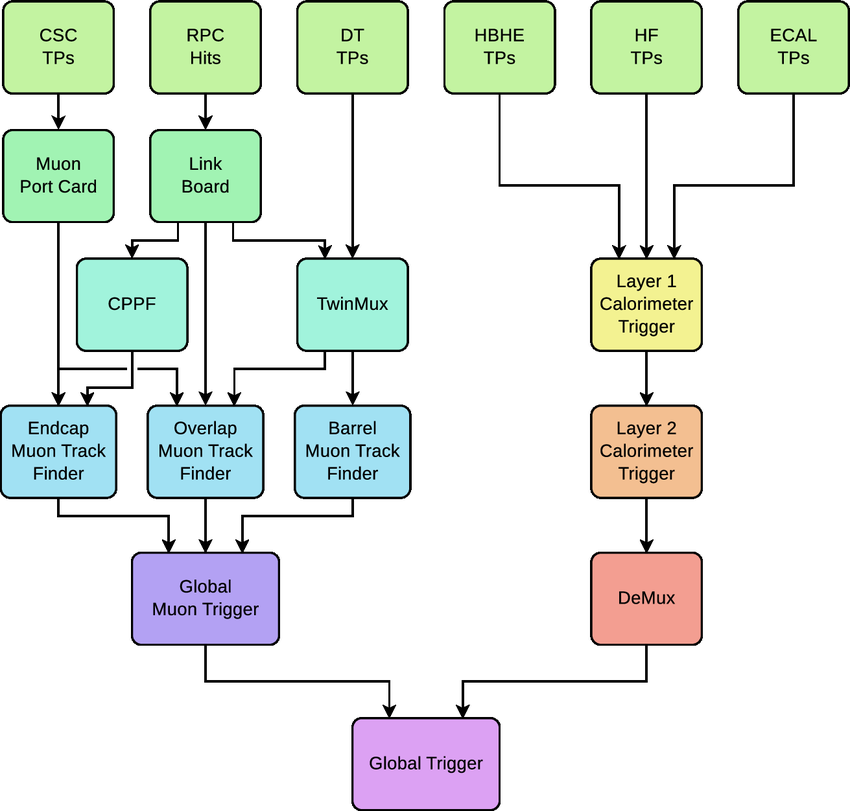
\includegraphics{Immagini/TriggerSystem.png}} 
    \end{column}
\end{columns}

\end{frame}


\section{Proprietà dei candidati Muoni}
\subsection{Validazione delle Trigger  Superprimitives}

\begin{frame}{Trigger Superprimitives}


\begin{columns}

    \begin{column}{0.5\textwidth}
     \centering
        %\scalebox{0.2}{\includegraphics{Immagini/TriggerNic.png}} 
    \end{column}


    \begin{column}{0.5\textwidth}
        \centering
        %\scalebox{0.2}{\includegraphics{Immagini/TriggerNic.png}} 
    \end{column}
\end{columns}

    
\end{frame}



    
    
\end{document}